%!TEX root = ../main.tex

\chapter{Introducción}
\label{intro}

En las últimas dos décadas distintas técnicas de ingeniería reversa del aprendizaje en humanos han inspirado con éxito distintos algoritmos de inteligencia artificial \cite{russell2002artificial}. Los avances recientes en las técnicas de aprendizaje profundo han logrado resultados notables en numerosos dominios como reconocimiento visual de objetos, el reconocimiento automático del habla, la búsqueda de respuestas y las traducciones automáticas \cite{lecun2015deep}. En la mayoría de estos enfoques, el resultado y el objeto del proceso de aprendizaje es una función estadística de reconocimiento de patrones específicos en los datos. Sin embargo, en muchas situaciones, el aprendizaje humano implica la construcción de modelos estructurados de conocimiento abstracto a partir de pocos datos, y este tipo de sistemas no han sido capaces de imitar esa habilidad \cite{lake2017building}.

¿Cómo pueden las personas adquirir un vasto universo de conceptos con muy poca exposición aparente? Una posible solución a este enigma, conocida como el problema de Platón ~\cite{chomsky1986knowledge, chomsky2006cognitive}, surge del aprendizaje automático probabilístico. Este enfoque está arrojando algo de luz sobre cómo los humanos pueden construir modelos y abstracciones bajo incertidumbre y a partir de datos escasos \cite{tenenbaum2011grow,ghahramani2015probabilistic}, y está renovando la hipótesis de Jerry Fodor que afirma que el pensamiento toma forma en una especie de lenguaje mental del pensamiento (LoT, por sus siglas en inglés) compuesto por un conjunto limitado de símbolos atómicos que se pueden combinar para formar estructuras más complejas siguiendo reglas combinatorias \cite{fodor1975language}.

Nuestra investigación se suscribe a uno de las líneas actuales del aprendizaje automático probabilístico conocido como programación probabilística, un esquema general para expresar modelos probabilísticos y métodos de inferencia como programas informáticos \cite{ghahramani2015probabilistic}. Esto significa que en nuestros modelos asumimos que el LoT es un lenguaje de programación capaz de generar programas para modelar conceptos en el mundo. Con nuestro trabajo pretendemos mejorar nuestro entendimiento del proceso de aprendizaje a partir de cuerpos ralos de datos y desarrollar nuevos métodos y algoritmos de programación probabilística para replicar esta notable capacidad humana. 

En la sección..... (acá se explicaría capítulo por capítulo)


\section{Teoría computacional de la mente}
\textbf{Explicar critica conexionismo y surgimiento teoría computacional de la mente.} \\
\textbf{Breve mención a críticas del conectivismo a partir del 80 (Fodor y Steven Pinker). Reversión al asociacionismo.}\\
\textbf{Explicar Simbólico}\\

"The infite use of finite means" (Humboldt's sobre el lenguaje)

1) How does abstract knowledge guide learning and inference from sparse data?
Bayesian inference in probabilistic generative models

2) What form does that knowledge take, across different domains and tasks?
Probabilities defined over richly structured symbolic representations: spaces, graphs, grammars, logical predicates

3) How is that knowledge itself constructed / updated / validated?
Hierarchical models, transfer learning, herramientas papers


Los investigadores han modelado estas categorías mentales o clases conceptuales con dos enfoques clásicos: en términos de similitud con un ejemplo genérico o prototipo \cite{rosch1999principles, nosofsky1986attention, rosch1976structural, rosch1975family} o basándose en una representación simbólica de reglas \cite{boole1854investigation, fodor1975language, gentner1983structure}.

Enfoques simbólicos como la hipótesis del \textit{lenguaje del pensamiento} (LoT, por sus siglas en ingés) \cite{fodor1975language}, afirman que el pensamiento toma forma en una especie de lenguaje mental, compuesto por un conjunto limitado de símbolos atómicos que pueden combinarse para formar estructuras más complejas. siguiendo reglas combinatorias.

\textbf{Explicar críticas a simbólico} \cite{blackburn1984spreading, loewer1991meaning, knowles1998language, aydede1997language} \\


\section{Lenguaje del pensamiento}

\textbf{Profundizar Fodor y Cognición. Aparición de Probabilistic Language of Thought}\\

A pesar de las críticas y objeciones, los enfoques simbólicos en general --- y la hipótesis de LoT en particular --- han ganado una atención renovada con resultados recientes que podrían explicar el aprendizaje a través de diferentes dominios como inferencia estadística sobre un espacio de hipótesis estructurado composicionalmente \cite{tenenbaum2011grow, piantadosi2016four}.

El LoT no es necesariamente único. De hecho, la forma que adopta se ha modelado de muchas formas diferentes según el dominio del problema: aprendizaje de conceptos numéricos \cite{piantadosi2012bootstrapping}, aprendizaje de secuencias \cite{marie2016, yildirim2015learning, romano2013language}, aprendizaje de conceptos visuales \cite{ellis2015unsupervised}, aprendizaje de teorías \cite{ullman2012theory}, etc.

Si bien los marcos pueden diferir en cómo se puede implementar un LoT computacionalmente, todos comparten la propiedad de estar construidos a partir de un conjunto de símbolos y reglas atómicos mediante los cuales se pueden combinar para formar expresiones nuevas y más complejas. 

La mayoría de los estudios de LoT se han centrado en el aspecto compositivo del lenguaje, que se ha modelado dentro de un \cite{tenenbaum2011grow} bayesiano o un marco \cite{marie2016, goldsmith2002probabilistic, romano2013language, goldsmith2001unsupervised} de longitud mínima de descripción (MDL).

El método común es definir una gramática con un conjunto de producciones basadas en operaciones que son intuitivas para los investigadores y luego estudiar cómo diferentes procesos de inferencia coinciden con patrones regulares en el aprendizaje humano. Un estudio reciente \cite{piantadosi2016logical} pone el foco en el proceso de cómo elegir empíricamente el conjunto de producciones y cómo diferentes definiciones de LoT pueden crear diferentes patrones de aprendizaje. 


\subsection{Gramáticas}


\textbf{Explicar gramáticas}\\
\textbf{Explicar diferencia entre sintaxis y semántica}\\

El proyecto de análisis bayesiano del aprendizaje de conceptos de modelos LoT utilizando inferencia bayesiana en un espacio de hipótesis estructurado gramaticalmente \cite{goodman2008rational}. Cada propuesta de LoT suele formalizarse mediante una gramática libre de contexto $ \gram $ que define las funciones o programas válidos que se pueden generar, como en cualquier otro lenguaje de programación. Un programa es un árbol de derivación de $ \gram $ que debe interpretarse o ejecutarse de acuerdo con una semántica determinada para obtener una descripción real del concepto en la tarea cognitiva en cuestión. Por lo tanto, cada concepto es luego representado por cualquiera de los programas que lo describen y se define un proceso de inferencia bayesiano para inferir de los datos observados la distribución de programas válidos en $ \gram $ que describen los conceptos.

\subsection{Composición}
Los lenguajes combinatorios pueden describir un vasto conjunto de conceptos a partir de un pequeño conjunto de primitivas. Esto se puede entender en un ejemplo relativamente simple en el dominio de las formas. Un lenguaje combinatorio y simbólico similar a Logo ~\cite{abelson1974logo} puede combinar operaciones como "mover", "pluma arriba", "pluma abajo" o "rotar" para generar un conjunto infinito de expresiones (o programas) que, cuando se evalúa, puede transmitir todo tipo de formas.

Un lenguaje que describe conceptos (como formas) también proporciona una noción natural de su complejidad \cite{kolmogorov1968three}. Un concepto es simple, relativo a ese lenguaje, cuando puede describirse mediante un programa corto. Por el contrario, es complejo cuando todas sus descripciones requieren una larga secuencia de instrucciones. Por ejemplo, en el caso del lenguaje Logo, un cuadrado puede simplemente instruirse como un bucle de cuatro desplazamientos seguidos de rotaciones de 90 grados. En este lenguaje, el icono de un rostro se implementará mediante un programa mucho más largo y, por lo tanto, será más complejo. Sin embargo, este concepto sería más sencillo cuando se describiera en un lenguaje en el que el icono de un rostro (o los símbolos de nariz, boca, etc.) estén disponibles como primitivos en el lenguaje.

En el dominio de los conceptos booleanos, se estudió una amplia gama de variedades lógicas de conceptos en ~\cite{feldman2003simplicity}, revelando una ley sorprendentemente simple: la dificultad subjetiva de un concepto booleano para un aprendiz humano es directamente proporcional a la longitud del programa compatible más corto en el lenguaje de la lógica proposicional (es decir, variables booleanas combinadas con los operadores \textit{and}, \textit {or} y \textit{not}). Este resultado puede sugerir que el LoT humano está equipado con reglas y símbolos similares a los que se encuentran en la lógica proposicional. De hecho, la correlación entre la dificultad subjetiva de los conceptos y su complejidad se ha utilizado como vehículo general para estudiar el LoT humano en varios dominios ~\cite{piantadosi2016logical, leeuwenberg1971perceptual, amalric2017language, romano2018, lupyan2007language}. Aunque a menudo está implícito, la estrategia general es (\textit{1)} asumir un idioma; (\textit{2)} encontrar el programa compatible más corto para algunos conceptos en ese idioma; (\textit{3)} comparar la duración de estos programas con la dificultad subjetiva de los conceptos; y finalmente (\textit{4)} repetir este proceso para varios idiomas dentro de un universo de posibles candidatos y elegir el idioma que mejor se ajuste en \textit{(3)}. Como se mencionó anteriormente, la longitud del programa depende de las primitivas del lenguaje en el que está escrito este programa, por lo que diferentes lenguajes hacen diferentes predicciones.

Una pregunta natural, sin embargo, es si las primitivas de una LoT son universales --tanto a través de diferentes individuos como a lo largo del desarrollo-- o si, en cambio, el repertorio semántico de un lenguaje es dinámico y está moldeado por la experiencia. De hecho, es probable que nuestra capacidad para representar automáticamente conceptos booleanos de manera sucinta no se deba a un lenguaje proposicional eficiente innato en nuestra mente. En cambio, proponemos que esta capacidad surge como un subproducto de nuestro cerebro que aprende rápidamente representaciones eficientes de los conceptos que generalmente encontramos en la vida cotidiana. 

Nuestra pregunta de investigación es: ¿con qué rapidez podemos adaptar nuestros mecanismos de aprendizaje cuando nos encontramos con un nuevo dominio en el que nuestras representaciones a priori ya no son eficientes? Examinamos la hipótesis de que los humanos tienen la capacidad de recombinar rápidamente proposiciones en su LoT, agregando nuevas primitivas a su lenguaje. En otras palabras, ese aprendizaje conduce a un proceso de compilación de rutinas en funciones dentro de el LoT.

En el ejemplo del lenguaje Logo se puede imaginar que si las producciones que dibujan cuadrados son muy frecuentes, sería eficaz dedicar un nuevo símbolo a esta producción. El nuevo símbolo "cuadrado" es una construcción jerárquica de "segundo orden" de las primitivas de "primer orden" del lenguaje. Tiene un costo (de incrementar el léxico del lenguaje) pero en el nuevo lenguaje, dibujar un cuadrado puede ser instanciado con un programa muy corto (es decir, "cuadrado") y por lo tanto usa menos memoria. De hecho, un lenguaje de nivel superior nos permite alcanzar un nivel superior de abstracción al liberar la memoria y el poder de procesamiento, haciendo así pensables pensamientos más complejos ~\cite{minsky1967computation, murphy1988comprehending}.

La mayor parte del trabajo en la literatura sobre LoT, aunque incluye naturalmente un mecanismo de aprendizaje, tiende a acercarse al LoT como un sistema estable que deben descubrir los experimentadores, que prueban diferentes plantillas candidatas y seleccionan la que mejor se ajusta a los datos después del entrenamiento ~\cite{goodman2008rational, kemp2012exploring, piantadosi2016logical}. Aún así, queda por descubrir cómo las diferentes trayectorias de la experiencia pueden dar forma a la adquisición de manera diferente y pueden cambiar constantemente el repertorio de un LoT después de cada exposición.


\section{Teoría algorítmica de la información}

\widesanti{De esto que sigue podés dejar todo, algo o eliminarlo por completo}

Cuando vemos las cadenas de 26 bits
\begin{align*}
\sigma_1 &= 10101010101010101010101010,\\
\sigma_2 &= 00100100001111110110101010, \\
\sigma_3 &= 11011010010000110101111010,
\end{align*}
tenemos la sensación de que la $\sigma_2$ y la $\sigma_3$
son {\em más difíciles} o {\em más complejas} que $\sigma_1$. Sin embargo, en términos de
teoría de la medida, cada una es igual de probable, si provienen de una fuente que emite bits 
con probabilidad uniforme. 
La intuición es que las cadenas sencillas tienen patrones reconocibles (como $\sigma_1$) mientras
que las más complejas no (o al menos no tienen patrones simples). 
En efecto, con la información adicional de que $\sigma_2$ se compone de los dígitos de 
la expansión fraccionaria de $\pi$ en binario, esta secuencia --intuitivamente-- se vuelve de inmediato más simple que antes, puesto que aparece una regla para producirla. Lo cierto es que $\sigma_3$ fue generada tirando una moneda y anotando 0 si salía cara y 1 si salía ceca. Nuestra intuición también nos dice que lo más probable es que una cadena generada mediante este procedimiento no tenga patrones reconocibles.

Entender por qué
algunas secuencias parecen aleatorias o complejas mientras que otras no, es una cuestión
profunda y fundamental. Desde principios del siglo {\small XX} se
empezó a pensar en este problema. Pero cómo transformar nuestra
intuición de `lo complejo' en una definición matemática, y cómo calibrar esta noción, no fue una tarea fácil. 
Al final, las definiciones que se
encontraron terminaron estando todas muy relacionadas con los métodos efectivos y con la 
teoría de la computación.

% La {\em teoría de largo de programa} define una noción de
% complejidad que clasifica las cadenas de 0s y 1s según la longitud
% del programa más corto que las computa. Esta complejidad se llama
% {\em complejidad de Kolmogorov}. Las cadenas más complejas son
% aquellas que requieren un programa esencialmente de igual longitud
% que la cadena misma, y las más sencillas son las que admiten un
% programa sustancialmente más corto. 

La {\em teoría algorítmica de la información}, también
conocida como {\em teoría de largo de programa} fue iniciada
independientemente en la década del 60 por Kolmogorov \cite{kolmogorov1965three},
Solomonoff \cite{solomonoff1964formal} y Chaitin \cite{chaitin1969length}. 
Esta teoría define una
noción de complejidad de cada palabra teniendo en cuenta la longitud
del programa más corto que computa esa palabra. Así, los programas
son vistos como {\em descripciones algorítmicas} de palabras. De
entre todas las descripciones de una palabra podemos tomar la que
tiene menor longitud como una medida de su complejidad. Una palabra
$\sigma$ es simple, es decir, tiene baja complejidad, si su
complejidad es sustancialmente menor que la longitud de $\sigma$; y
una palabra es compleja si su descripción algorítmica es tan larga
como la longitud misma de $\sigma$. La gran mayoría
de las palabras tiene complejidad alta. La función que asocia a cada
palabra $\sigma$ la longitud del programa más corto que devuelve
$\sigma$ como salida (cuando es ejecutado en una cierta máquina
universal de referencia) se llama {\em complejidad de Kolmogorov} o
{\em complejidad de largo de programa}.

Debe
observarse que en esta definición --todavía informal-- 
de complejidad de Kolmogorov hay
un lenguaje de descripción subyacente. La teoría algorítmica de la información
toma a los lenguajes de programación como lenguaje de descripción. Sin embargo, 
hay que notar que una definición en la misma dirección puede aplicarse para 
otros objetos en el rol de las cadenas binarias (por ejemplo, conjuntos de valuaciones 
Booleanas) y otros lenguajes de descripción en el rol de lenguajes de programación
(por ejemplo, fórmulas de la lógica proposicional). En todo caso, es fundamental
que los lenguajes de descripción tengan una semántica formal para evitar paradojas
como la de Berry, que propone definir $n$ como el primer número natural que no sea 
descriptible con menos de 90 caracteres. Por definición la descripción más corta de $n$ debe tener 
al menos 91 letras, y sin embargo su definición ``el primer número natural que no sea 
descriptible con menos de cincuenta caracteres'' evidentemente lo describe y tiene 83 caracteres.

Desde el punto de 
vista teórico, la riqueza de la Complejidad de Kolmogorov
aparece cuando el lenguaje de programación subyacente es 
Turing completo, 
es decir, es capaz de definir cualquier función parcial
computable. En la teoría, los lenguajes de programación se
formalizan con máquinas de Turing y los lenguajes Turing completos
como máquinas universales. 
Cuando el dominio de los programas (máquinas) es libre de prefijos (es decir, no hay dos programas
que terminan en dónde uno es una extensión propia del otro)
hablamos de complejidad de Kolmogorov {\em libre de prefijos}
(denotada con $K$) y cuando no se impone ninguna restricción en
el dominio, hablamos de complejidad de Kolmogorov plana (denotada
con $C$). La necesidad de trabajar con dominios libres de prefijos es
técnica y está vinculada con la utilidad de la complejidad de Kolmogorov 
para definir nociones de aleatoriedad.
% Esta noción de complejidad es absoluta, pues si bien existe una
% complejidad distinta por cada máquina universal subyacente, todas
% estas son iguales salvo una constante aditiva \cite{C94,LV97}.

A continuación veremos las definiciones formales de la Complejidad de Kolmogorov y de los
principales elementos de la Teoría algorítmica de la información.

% Los orígenes del estudio de la aleatoriedad algorítmica se remontan
% a los trabajos de von Mises de principios del siglo {\small XX}
% \cite{M19}, en dónde argumentaba que las secuencias aleatorias deben
% tener ciertas propiedades de estocasticidad desde el punto de vista
% de la teoría clásica de la probabilidad.

% Intuitivamente una secuencia es aleatoria cuando carece de
% estructura o regularidad, en otras palabras, cuando no tiene
% patrones reconocibles. Uno querría definir a las secuencias
% aleatorias como aquellas que  son indistinguibles del resultado de
% arrojar infinitas veces una moneda y anotar $0$ si sale cara o $1$
% si sale ceca. Así, las secuencias
% $$
% 00000000000000000000\dots \mbox{\quad o \quad }
% 10101010101010101010\dots
% $$
% no parecen aleatorias porque se pueden reconocer marcados patrones.
% En cambio, uno siente que una secuencia como
% $$
% 10010111010111100101\dots
% $$
% es aleatoria porque es difícil reconocer patrones. Las
% clarificaciones de precisamente qué constituye lo aleatorio fueron
% hechas recién pasada la mitad del siglo {\small XX}.

% Martin-L\"of \cite{M66} introdujo una noción de aleatoriedad basado
% en tests estadísticos. La idea es que una secuencia aleatoria
% debería pasar todo posible test estadístico razonable. Martin-L\"of
% formaliza esta noción de {\em test estadístico razonable} como un
% tipo particular de conjuntos efectivos de medida $0$. Su propuesta
% es que una secuencia es aleatoria cuando evita (es decir, logra
% escapar de) todos esos conjuntos efectivos de medida $0$.

% Independientemente, Chaitin \cite{C76b} introdujo la noción de
% aleatoriedad en términos de la complejidad de Kolmogorov (en
% realidad, de una variante de esa complejidad que se denomina
% complejidad {\em libre de prefijos}): las secuencias
% Chaitin-aleatorias son aquellas cuyos segmentos iniciales son {\em
% incompresibles}. Es decir, la complejidad de Kolmogorov de los
% primeros $n$ dígitos de la secuencia es mayor que $n$ menos una
% constante fija.


% Es interesante el hecho de que la idea de {\em procedimiento
% efectivo} está involucrada en todas las definiciones de aleatoriedad. 

\subsection{Complejidad de Kolmogorov}
\widesanti{Introducir la noción formal. Empezar por $K_M$, con $M$ una máquina específica. Luego la $K_U$, con $U$ universal. Dar la versión plana y la libre de prefijos (puesto que esa es la que se usa para el coding theorem). Dar el coding theorem sin demo, solo enunciado.}


\widesanti{Podés retomar los ejemplos de $\sigma_1$, $\sigma_2$, $\sigma_3$ de más arriba y explicar que programas cortos los generan. O podés exagerarlos a más bits. Esto da idea de la diferencia entre la descripción y lo descripto (aunque es cierto que la tesis es sobre aprendizaje con POCOS datos...) Para los programas, alcanza con un pseudo código o incluso descripción informal, pero dado que es una tesis en computación, también podés usar un lenguaje verdadero, Python, ponele. Podés también poner alguna otra cadena, $\sigma_4$ en donde haga falta anidar loops, porque eso es importante para el cap 2. Por ejemplo, 000111000 1 000111000 1 000111000}


\widesanti{Esto que sigue es parte de mi tesis. Podés simplemente traducirlo y dejarlo tal cual. 
Ojo que hay cosas de más... y muchos comandos latex :P}


In this section we introduce the plain and \pfree \kolcomp and we
mention some known results and standard notation that will be used
repeatedly in the rest of this thesis. Some other important
results will be introduced when necessary.

In algorithmic information theory, programs are regarded as
algorithmic descriptions of strings. As we mentioned in
section~\ref{intro:sec:recursion}, we say that a program $\pra$
{\em $\M$-describes} a string $\sta$ when it is executed in a
Turing machine $\M$ and produces $\sta$ as output. In general
there is more than one program describing the same output $\sta$.
The idea of the \kolcomp introduced in~\cite{kolmogorov1965three,solomonoff1964formal,chaitin1975theory} is to
take the length of a shortest description as a measure of the
complexity of the string.

\begin{definicion}[Plain \kolcomp]\label{intro:def:plainC}
$\CM\colon\words \to \nat$, 
the {\em plain
\kolcomp with respect to the Turing machine $\M$}, is defined as
$$
\CM(\sta)=
    \begin{cases}
    \min \{\len{\pra}\colon \M(\pra)=\sta \} & \textrm{if $\sta$ is in the range of $\M$};\\
    \infty & \textrm{otherwise.}
    \end{cases}
$$
\end{definicion}
If we restrict ourselves to partial \rec functions with \pfree
domain, we can think of  {\em
\pfree Turing machines} (independently introduced by
Levin~\cite{L71,L73}, Schnorr~\cite{S71} and Chaitin~\cite{chaitin1975theory})
as the formalism to compute them. Chaitin thought of a convenient
device to compute exactly all \pfree machines. This device is just
like a classical Turing machines but the input tape is a bit
primitive: the input head moves only to the right and there is no
blank end-marker delimiting the end of the input. So a \pfree
machine starting with the input head in the first bit of the input
$\pra$ may eventually try to read beyond the end of $\pra$ and if
this happens, it simply crashes (i.e.\ it becomes undefined) and
it stays in that error state forever. Therefore, for a \pfree
machine $\M$ to succeed in the computation, it needs to somehow
figure out by itself where the end of the input is.
% no extension of a valid program is a valid program.
This is the reason why this device is sometimes called {\em
self-delimiting} machine. In this model, if a given input is
defined, all its extensions are undefined. It can be shown that
this restricted architecture of Turing machines compute exactly
all partial \rec functions with \pfree domain. The {\em the \pfree
\kolcomp}~\cite{levin1974laws,G74,chaitin1975theory} is defined in the same way as in
Definition~\ref{intro:def:plainC} but relative to \pfree
machines:

\begin{definicion}[\Pfree \kolcomp]\label{intro:def:prefixK}
\index{Program-size complexity@\kolcomp!prefix@\pfree}
\glossary{$\KM$}$\KM\colon\words \to \nat$, the {\em \pfree
\kolcomp with respect to the \pfree machine $\M$}, is defined as
$$
\KM(\sta)=
    \begin{cases}
    \min \{\len{\pra}\colon \M(\pra)=\sta \} & \textrm{if $\sta$ is in the range of $\M$};\\
    \infty & \textrm{otherwise.}
    \end{cases}
$$
\end{definicion}
The two complexity functions $\C$ and $\K$ have been used for
different purposes
% Under some situations it is more adequate to use \pfree \kolcomp instead of plain \kolcomp
(for more details, see~\cite{DHBook} and~\cite{LV97}). In this
thesis we will mainly use \pfree \kolcomp, but in some sections we
will also work with the plain version.

There are two traditions of notation in the \kolcomp community as
regards the plain/\pfree versions: the $C$/$K$ tradition and the
$K$/$H$ tradition. In recent years it seems that the $C$/$K$
notation appears more often in both the complexity and the
recursion theory literature. In this document, we follow the
$C$/$K$ notation.

\bigskip

Observe that it does not matter if the list in
(\ref{intro:eqn:enumPRfunctions}) is an enumeration of all
classical machines or all \pfree machines (both have a finite
table of instructions, so they can be effectively listed). The
machine $\V$ defined in (\ref{intro:eqn:usualUniversalMachine})
exists in both cases and in the second, $\V$ is also \pfree.


The classical notion of universality from computability theory is
redefined in the algorithmic information theory. We will use the
word {\em \opt} for denoting machines like $\V$ defined in
(\ref{intro:eqn:usualUniversalMachine}) that somehow simulate
every other machine at no noticeable extra cost in the length.

\begin{definicion}[\Optity]\label{intro:def:optimal}
\index{Turing!machine!universal@\opt} $\U$ is a {\em \opt} \pfree
(resp.\ classical) Turing machine if and only if
$$
(\forall e)(\exists c_e)(\forall \pra)(\exists \prb_{e,\pra})\,
[\U(\prb_{e,\pra})=\T_e(\pra) \ \wedge \len{\prb_{e,\pra}}\leq
\len{\pra}+c_e],
$$
where $\T_0,\T_1,\T_2,\dots$ is an enumeration of all the \pfree
(resp.\ classical) Turing machines
\end{definicion}

When working with oracles, $\U$ will be \opt if it may simulate
{\em any} other machine with {\em any} oracle, so it is {\em
universally universal}. In the case of an \pfree \opt machine,
$\U^A$ will be \pfree for all $A\subseteq\nat$.

In general we use the same letter $\U$ for denoting both a
classical \opt machine and a \pfree \opt machine; it will always
be clear from the context which one we refer to. In~\cite{chaitin1975theory}
Chaitin called these machines {\em optimal universal}, because
they permit us to define the \kolcomp in an {\em optimal} way:

\begin{teorema}[Invariance]\label{intro:thm:invariance}
\index{Invariance Theorem} If $\U$ is \opt \pfree (resp.\
classical) Turing machine then for any \pfree (resp.\ classical)
Turing machine $\M$ there is a constant $c$ such that for all
$\sta\in\words$, $\KU(\sta)\leq \KM(\sta)+c$ (resp.\
$\CU(\sta)\leq \CM(\sta)+c$).
\end{teorema}

Hence for any two \pfree \opt machines $\U$ and $\V$, the \pfree
\kolcomp with respect to $\U$ and $\V$ is the same up to an
additive constant, i.e.\ there is some constant $c$ such that
$\abs{\KU(\sta)-\KV(\sta)}\leq c$ for any $\sta\in\words$. Of
course the same is true for classical machines and $\C$. If there
is no need to refer to the underlying \opt machine $\U$, one just
writes \glossary{$\K$}$\K$ for $\KU$ and \glossary{$\C$}$\C$ for
$\CU$. In this way, $\K$ and $\C$ become an {\em absolute} measure
of the complexity of the strings.

To illustrate some useful application of the Invariance Theorem,
let us see some upper bounds for $\K$ and $\C$. Imagine a
classical machine $\M$ that reads the input $\sta$ and writes
$\sta$ as its own output. Then $\CM(\sta)=\len{\sta}$ for all
$\sta\in\words$ and by the Invariance
Theorem~\ref{intro:thm:invariance} this shows that for all $\sta$,
$\C(\sta)\leq \len{\sta}+c$ for some constant $c$. With \pfree
machines the situation is a bit different because the machine has
to discover by itself where the end of the input is. Suppose $\U$
is any \opt \pfree machine and suppose $\pra_\sta$ is a minimal
$\U$-description of $\len{\sta}$. This just means that
$\U(\pra_\sta)=\len{\sta}$ and $\len{\pra_\sta}=\K(\len{\sta})$.
Then there is a \pfree machine $\N$ that with input
$\pra_\sta\sta$ can do the following: fist simulate $\U$ step by
step. Each time $\U$ asks for reading one more bit, $\N$ obeys and
reads from its own input. Eventually $\U$ will read the whole
$\pra_\sta$ and will terminate with $\U(\pra_\sta)=\len{\sta}$ as
output. Now $\N$ (which is still running) knows that exactly
$\len{\sta}$ more bits need to be read from the input. So $\N$
reads $\len{\sta}$ bits from the input and recovers $\sta$.
Afterwards, $\N$ writes $\sta$ in the output and terminates. This
shows that $\N(\pra_\sta\sta)=\sta$. Of course, if the input is
wrong, the computation may go wrong, for example $\N$ can try to
read beyond the end of the input and then crashes. However, when
the input is of the form $\pra_\sta\sta$, $\N$ always outputs
$\sta$. By the invariance Theorem \ref{intro:thm:invariance} this
shows that $\K(\sta)\leq \len{\pra_\sta\sta} + d =
\K(\len{\sta})+\len{\sta}+d$ for some constant $d$. These upper
bounds on $\C$ and $\K$ will be repeatedly used in the thesis. We
will also use that for any $n$ there is a string $\sta$ of length
$n$ such that $\K(\sta)\geq n$. This is true because there are at
most $2^n-1$ programs of length less than $n$ but $2^n$ strings of
length $n$. The same holds for $\C$. In fact,
Chaitin~\cite{chaitin1975theory,C87b} showed that there is a constant $c$ such
that for all $d\in\nat$ and all $n$
$$
\size{\{ \sta \colon \len{\sta}=n \wedge \K(\sta)\leq n + \K(n)-d
\}} \leq 2^{n-d+c}
$$
This result is usually called \index{Counting Theorem}Counting
Theorem, tells us that only a small fraction of all the strings of
length $n$ have \pfree \kolcomp below $n+\K(n)-d$, when we take
$d$ much bigger than $c$.
Observe that if we let $d=n-b$, we obtain
$$
\size{\{ \sta \colon \len{\sta}=n \wedge \K(\sta)\leq \K(n)+b
\}} \leq 2^{b+c}
$$
and this last upper bound depends on $b$ and $c$, but not on $n$.

As we explained in the last paragraph, one way to bound the
\kolcomp is to explicitly design specific machines, like $\M$ or
$\N$ and explain their behavior. Another powerful method to
implicitly build \pfree machines and upper bound the \pfree
\kolcomp is via a Kraft-Chaitin set. This method consists of an
effective interpretation of an inequality of Kraft~\cite{K49}:

\begin{definicion}[Kraft-Chaitin set]\label{intro:KCset}
\index{Kraft-Chaitin} A \ce\ set
$$
W=\{\pair{n_0}{\sta_0}, \pair{n_1}{\sta_1},
\pair{n_2}{\sta_2},\dots\},
$$
where $n_i\in\nat$ and $\sta_i\in \words$, is a {\em Kraft-Chaitin
set} if $\wt{W}\leq 1$, where \glossary{$\wt{W}$}$\wt{W}=
\sum_{i\in\nat} 2^{-n_i}$ is the {\em weight} of $W$. The pairs
enumerated into such a set $W$ are called {\em axioms}.
\end{definicion}

The Kraft-Chaitin Theorem can be found in Levin's
Thesis~\cite{L71} and in~\cite{levin1974laws}, Schnorr also included a
version of it in~\cite{S73} and Chaitin~\cite{chaitin1975theory} gave the first
proof explicitly for \pfree \kolcomp. This theorem states that
from a Kraft-Chaitin set $W$ like the one described in the above
Definition~\ref{intro:KCset}, we can effectively obtain a \pfree
machine $\M$ such that for each $i$ there is a $\pra_i$ of length
$n_i$ with $\M(\pra_i)\downarrow=\sta_i$, and $\M(\prb)\uparrow$
unless $\prb=\pra_i$ for some~$i$. Observe that the machine $\M$
is built in an implicit way: we only need to specify the lengths
of the programs we want. In particular, the Kraft-Chaitin Theorem
states that there is a constant $c$ such that for all $i$,
$\K(\sta_i)\leq\min\{m\colon\pair{m}{\sta_i}\in W\}+c$.

\bigskip

\subsection{El teorema de la codificación}

The complexity $\K$ is related with the probability that a \pfree
machine $\M$ outputs a given string $\sta$. This last magnitude is
defined as \glossary{$P$}
\begin{eqnarray}
P_{\M}(\sta)&=&\measure{\open{\{\pra\colon\M(\pra)=\sta\}}}\nonumber\\
&=&\sum_{\pra\colon\M(\pra)=\sta}2^{-\len{\pra}}.\label{intro:eqn:coding}
\end{eqnarray}
Clearly, for all $\sta$, $2^{-\K(\sta)}\leq P_{\U}(\sta)$, since a
shorter $\M$-description of $\sta$ already contributes to the sum
in equation (\ref{intro:eqn:coding}). The following result, due to
Levin \cite{levin1974laws}, G\'acs \cite{G74} and Chaitin, \cite{chaitin1975theory} known
as the {\em Coding Theorem}, states that the other inequality is
also true, except for a multiplicative constant

\begin{teorema}[\index{Coding Theorem}Coding Theorem]\label{intro:thm:coding} For each \pfree machine $\M$, one
may effectively find a constant $c$ such that $ (\forall
\sta\in\words)\ 2^{c-\K(\sta)}\geq P_{\M}(\sta). $
\end{teorema}
For more information in the Coding Theorem, see \cite{LV97} and
\cite{DHBook}.

\bigskip

\index{Program-size complexity@\kolcomp!\computable@\comp
approximation} Although $\K$ and $\C$ are not \comp functions,
they can be \recly approximated from above using the step by step
approximation of $\U$. \glossary{$\K_s$}$\K_s(\sta)$ is the
approximation at stage $s$ of $\K(\sta)$ defined by
$\K_s(\sta)=\min\{\len{\pra}\colon
\U_s(\pra)=\sta\}\cup\{\infty\}$. Observe that
$\K_s(\sta)\to\K(\sta)$ when $s\to\infty$.
 The same holds for
\glossary{$\C_s$}${\C_s}$.


Machines can be relativized to oracles. For any $\M^A$, a \pfree
machine $\M$ relativized to an oracle $A$, $\domain {\M^A}$ has to
be \pfree. The Definition~\ref{intro:def:prefixK} of \kolcomp can
be relativized to oracles:

\begin{definicion}[Relativized \pfree \kolcomp]\label{intro:def:prefixKwithOracle}
\index{Program-size complexity@\kolcomp!relativized}
\glossary{$\KM^A$}$\KM^A\colon\words \to \nat$, the {\em \pfree
\kolcomp with respect to the \pfree machine $\M$ and relative to
oracle $A$}, is defined as
$$
\KM^A(\sta)=
    \begin{cases}
    \min \{\len{\pra}\colon \M^A(\pra)=\sta \} & \textrm{if $\sta$ is in the range of $\M^A$};\\
    \infty & \textrm{otherwise.}
    \end{cases}
$$
\end{definicion}

Definition~\ref{intro:def:plainC} of $\CM$ also adapts
straightforwardly to \glossary{$\CM^A$}$\CM^A$. Again, when there
is no need to refer to the underlying \opt machine, we just write
\glossary{$\C^A$}$\C^A$ and \glossary{$\K^A$}$\K^A$. Having an
oracle $A$ gives more power for compressing strings, so $\K^A$ is
always smaller than $\K$ up to an additive constant. The same
holds for $\C^A$ and $\C$.




\subsubsection{Un lenguaje concreto: el lenguaje de geometría}

\widesanti{Pego acá esto por si sirve. Quizá tenga sentido dar la semántica formal, dado que nunca apareció en ningún lado y que el cap 2 lo necesita en su versión simplificada.}



We define a simple programming language called {\em language of geometry}, $\+LG$, whose programs describe mappings $\Sigma\to\Sigma^+$, for $\Sigma=\{0,\dots,7\}$.
A program $p$, on input $n\in\Sigma$ (regarded as a natural number), is represented as $p(n)$, and it is a nonempty string formed by symbols in $\Sigma$. The strings in $\Sigma^+$ should be better thought to represent paths along the points in a circle, as depicted in Figure \ref{fig:circle}. $\+LG$ will contain instructions that can navigate the circle from one point to another and then to another and so on, jumping from one point to another a fixed number of steps, both clockwise or counterclockwise, and using the reflection over some axes. It also contains some structures to repeat certain paths.

\begin{figure}[ht]
\begin{center}
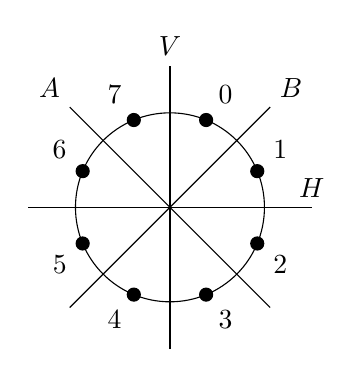
\begin{tikzpicture}[scale=.6]
\draw (-3,0) -- (3,0) node[above]{$H$};
\draw (0,-3) -- (0,3) node[above]{$V$};
\draw (-2.121320344,-2.121320344) -- (2.121320344,2.121320344) node[above right]{$B$};
\draw (2.121320344, -2.121320344) -- (-2.121320344,2.121320344) node[above left]{$A$};
\node at (0.765366865,  1.847759065) [circle,draw, scale=.5, fill, label=67.5:$0$]{};
\node at (1.847759065   , 0.765366865) [circle,draw, scale=.5, fill, label=22.5:$1$]{};
\node at (1.847759065   , -0.765366865) [circle,draw, scale=.5, fill, label=-22.5:$2$]{};
\node at (0.765366865   , -1.847759065) [circle,draw, scale=.5, fill, label=-67.5:$3$]{};
\node at (-0.765366865, -1.847759065) [circle,draw, scale=.5, fill, label=-112.5:$4$]{};
\node at (-1.847759065, -0.765366865) [circle,draw, scale=.5, fill, label=-157.5:$5$]{};
\node at (-1.847759065, 0.765366865) [circle,draw, scale=.5, fill, label=-202.5:$6$]{};
\node at (-0.765366865, 1.847759065) [circle,draw, scale=.5, fill, label=-247.5:$7$]{};
\draw (0,0) circle (2cm);
\end{tikzpicture}
\end{center}
   \caption{The symbols of $\Sigma$ around a circle, and the reflection axes.}\label{fig:circle}
\end{figure}


We first define the syntax of $\+LG$ and then introduce its formal semantics.

\paragraph{Syntax.}
The set of {\em instructions} is defined as
$$
\+I=\{+0,+1,+2,+3,-1,-2,-3,P,A,B,H,V\}.
$$
A {\em program} $p$ is a list of the form $[p_1,p_2,\dots,p_\ell]$, where each $p_i$ is either an instruction in $\+I$, or an expression of the form $q^s$, or $q^s\langle i\rangle$, or $q^s\{i\}$, where where $q$ is a program, $s$ is the decimal representation of some positive integer, and  $i\in\+I$.
%
%
%
%\begin{enumerate}
%\item an instruction in $\+I$
%\item an expression of the form $q^s$, where $q$ is a program and $s$ is the decimal representation of some positive integer
%\item an expression of the form $q^s\langle i\rangle$, where $q$ is a program, $s$ is the decimal representation of some positive integer, and  $i\in\Sigma$
%\item an expression of the form $q^s\{i\}$, where $q$ is a program, $s$ is the decimal representation of some posirive integer, and  $i\in\Sigma$
%\end{enumerate}


\paragraph{Semantics.}
The idea is that any program $p$ of $\+LG$ on input $n$ describes a string in $\Sigma^+$. The instructions in $\+I$ will allow us to navigate from a given point $n$ into another, and the expressions of the form $q^s$, or $q^s\langle i\rangle$, or $q^s\{i\}$ will represent three kind of loops, which will allow us to repeat a given pattern along the circle.

Let $p=[p_1,\dots,p_\ell]$ be a program of $\+LG$ and let $n$ be a number in $\{0,\dots,7\}$. We define the string $p(n)\in\Sigma^+$ recursively in the complexity of $p$:
\begin{itemize}
\item If $\ell=1$ and $p_1\in\+I$ then $p(n)$ is defined as follows:
	\begin{itemize}
	\item $[+0](n)\eqdef  n$ (no change)
	\item $[+1] (n) \eqdef   n+1 \mod 8$ (move 1 clockwise)
	\item $[-1] (n) \eqdef   n-1 \mod 8$ (move 1 counterclockwise)
	\item $[+2] (n) \eqdef   n+2 \mod 8$ (move 2 clockwise)
	\item $[-2] (n) \eqdef   n-2 \mod 8$ (move 2 counterclockwise)
	\item $[+3] (n) \eqdef   n+3 \mod 8$ (move 3 clockwise)
	\item $[-3] (n) \eqdef   n-3 \mod 8$ (move 3 counterclockwise)
	\item $[P](n)\eqdef  4+n \mod 8$ (move to the opposite point)
	\item $[H](n)\eqdef  3-n \mod 8$ (reflect over $H$)
	\item $[V](n)\eqdef  7-n \mod 8$ (reflect over $V$)
	\item $[A](n)\eqdef  5-n \mod 8$ (reflect over $A$)
	\item $[B](n)\eqdef  1-n \mod 8$ (reflect over $B$)
	\end{itemize}

\item If $\ell=1$ and $p_1\notin\+I$ then $p(n)$ is recursively defined as follows:

	\begin{itemize}
	\item If $p_1=q^s$, then
	$$
	p(n)\eqdef q(n_0)\dots q(n_{s-1}),
	$$
	where $n_0\eqdef n$ and $n_{k+1}$ is the last symbol of $q(n_k)$. In other words, $q^s$ on input $n$ represents a path given by:
	%
	\begin{quote}\em
	start in $n$ and repeat $s$ times the path represented by $q$.
	\end{quote}
	
	\item if $p_1=q^s\langle i\rangle$ and  $q(n)=x^0_1\dots x^0_k$ (for $x^k_j\in\Sigma$), then
	$$
	p(n)\eqdef x^0_1\dots x^0_k \ x^1_1\dots x^1_k \dots x^{s-1}_1\dots x^{s-1}_k,
	$$
	where $x^{k+1}_j\eqdef [i](x^k_j)$. In other words, $q^s\langle i\rangle$ on input $n$ represents a path given by:
	%
	\begin{quote}\em
	follow the path represented by $q$ starting in $n$. Say this is path $\sigma_0$. Then construct a path $\sigma_1$ which consists of applying $i$ to each single point of $\sigma_0$. Repeat this until you reach $\sigma_{s-1}$
	\end{quote}
	
	\item if $p_1=q^s\{i\}$ and  $q(n)=x_1\dots x_k$ (for $x_j\in\Sigma$), then
	$$
	p(n)\eqdef q(n_0)\ q(n_1)\dots q(n_{s-1}),
	$$
	where $n_0\eqdef n$ and $n_{k+1}\eqdef [i](n_k)$. In other words, $q^s\{ i\}$ on input $n$ represents a path given by:
	%
	\begin{quote}\em
	repeat $s$ times the following:  starting in $n$, follow the path represented by $q$, and set $n:=[i](n)$.
	\end{quote}
	
	
	
	\end{itemize}
	



\item Suppose $\ell>1$ and let $m$ be the last symbol of $p_1(n)$. We define
$$
p(n)\eqdef p_1(n) \ [p_2,\dots,p_\ell](m).
$$
%that is, the concatenation of $[p_1,\dots,p_{k-1}](n)$ and $p_k(m)$.

\end{itemize}

\paragraph{Examples.}
Let us see some examples:

\begin{itemize}
\item $[+1,-1](1)=21$

\item $[+0]^4(3)$ is the concatenation of $[+0](3)$ (which is $3$), $[+0](3)$, $[+0](3)$ and $[+0](3)$, i.e.\ $[+0]^4(3)=3333$.

\item $[+1]^4(0)$ is the concatenation of $[+1](0)$ (which is 1), $[+1](1)$ (which is 2), $[+1](2)$ (which is 3) and $[+1](3)$ (which is 4), i.e.\ $[+1]^4(0)=1234$.

\item $[+1,-1]^3(1)$ is the concatenation of $[+1,-1](1)$ (which is $21$), $[+1,-1](1)$ and  $[+1,-1](1)$, i.e.\  $[+1,-1]^3(1)=21212121$.

\item $[[+1]^4,[-2,[+1]^3]^2](0)$ is the concatenation of $[+1]^4(0)$ (which is $1234$) and $[-2,[+1]^3]^2(4)$. Now this one last is the concatenation of $[-2,[+1]^3](4)$ (which is $2345$) and $[-2,[+1]^3](5)$ (which is $3456$). In total we have $[[+1]^4,[-2,[+1]^3]^2](0)=123423453456$.

\item $[[[+1]^4]^3\langle +1\rangle ](0)$ is the concatenation of $[[+1]^4](0)$ (which is $1234$), $[+1](1)\ [+1](2)\ [+1](3)\ [+1](4)$ (which is $2345$), and $[+1](2)\ [+1](3)\ [+1](4)\ [+1](5)$ (which is $3456$). In total, we have $[[[+1]^4]^3\langle +1\rangle ](0) = 123423453456$.

\item $[[[+1]^4]^2\langle B\rangle](0)$ is the concatenation of $[[+1]^4](0)$ (which is $1234$) and $[B](1)\ [B](2)\ [B](3)\ [B](4)$ (which is $0765$). In total we have $[[[+1]^4]^2\langle B\rangle](0) = 12340765$.

\item $[[[V]^2]^4\{-1\}] (3)$ is the concatenation of $[[V]^2](3)$ (which is $43$), $[[V]^2](n_1)$ (for $n_1=[-1](3)=2$, which is $52$), $[[V]^2](n_2)$ (for $n_2=[-1](n_1)=1$, which is $61$), and $[[V]^2](n_3)$ (for $n_3=[-1](n_2)=0$, which is $70$). In total we have $[[[V]^2]^4\{-1\}] (3)= 43526170$.
\end{itemize}


\paragraph{Complexity.}
We define a Kolmogorov complexity relative to $\+LG$, that is, a measure of succinctness of a given string $\sigma\in\Sigma^+$ when the language of description is $\+LG$. Those strings which admit a small program describing it will have small complexity, and those strings which can only be described by large programs will have high complexity.

Before defining formally the notion of complexity, we need to formalize the idea of {\em size} of a program. Let $p=[p_1,\dots,p_\ell]$ be a program.
With $|p|$ we denote the {\em size} of $p$ . Roughly, $|p|$ is the number of letters needed to write down $p$. Formally, $|p|$ is defined as follows:
%
\begin{itemize}
\item If $\ell=1$ and $p_1\in\+I$ then $|p|\eqdef 2$.

\item If $\ell=1$ and $p_1\notin\+I$ then $|p|$ is recursively defined as follows:
%
	\begin{itemize}
	\item If $p_1=q^s$, then $|p|\eqdef |q|+\lceil \log s\rceil$
	\item if $p_1=q^s\langle i\rangle$ or $p_1=q^s\{ i\}$, then $|p|\eqdef |q|+\lceil \log s\rceil+|[i]|$
%	\item if $p_1=q^s\{ i\}$, then $|p|\eqdef |q|+\lceil \log s\rceil+|[i]|$
	\end{itemize}

\item If $\ell>1$ then $|p|\eqdef |p_1|+|[p_2,\dots, p_\ell]|$
\end{itemize}

Let $\sigma\in\Sigma^+$. We define the {\em complexity} of $\sigma$, notated $K(\sigma)$, as the size of the smaller program which on input $0$ describes $\sigma$, that is,
%
%For a given string $\sigma\in\Sigma^+$ we define the {\em complexity of $\sigma$ wrt $j\in\{0,\dots,7\}$}, notated $K_j(\sigma)$ as the size of the shortest program $p$ such that $p(j)=\sigma$.
$$
K(\sigma)\eqdef \min\{|p|\colon p(0)=\sigma\}.
$$
In Figure \ref{fig:strings} we show the complexity of some strings $\sigma$ and all programs $p$ such that $p(0)=\sigma$ and $|p|=K(\sigma)$.

\begin{figure}
\noindent{\small 
\begin{tabular}[t]{p{11em} p{11em} p{11em} p{11em}}
%
\begin{tabular}[t]{|p{10em}|}\hline
\bf Repeat+1\\
$01234567$\\
$K=5$\\
\hline
$[+0,[+1]^7]$\\
$[[+0]^8\langle +1\rangle ]$\\
$[[+0]^8\{+1\}]$
\\\hline\end{tabular}
&
\begin{tabular}[t]{|p{10em}|}\hline
\bf Repeat+2\\
$02460246$\\
$K=5$\\
\hline
$[+0,[+2]^7]$\\
$[[+0]^8\langle +2\rangle ]$\\
$[[+0]^8\{+2\}]$
\\\hline\end{tabular}
&
\begin{tabular}[t]{|p{10em}|}\hline
\bf Alternate\\
$0213243546576071$\\
$K=7$\\
\hline
$[[+0,+2]^8\langle+1\rangle]$\\ 
$[[+0,+2]^8\{+1\}]$
\\\hline\end{tabular}
&
\begin{tabular}[t]{|p{10em}|}\hline
\bf 2points\\
$02020202$\\
$K=7$\\
\hline
$[[+0,+2]^4\langle +0\rangle ]$\\
$[[+0,+2]^4\{+0\}]$
\\\hline\end{tabular}
\\
\\
\begin{tabular}[t]{|p{10em}|}\hline
\bf 2arcs\\
$01237654$\\
$K=8$\\
\hline
$[[+0,[+1]^3]^2\langle V\rangle ]$\\
$[[[+0]^4\langle +1\rangle ]^2\langle V\rangle ]$\\
$[[[+0]^4\{+1\}]^2\langle V\rangle ]$
\\\hline\end{tabular}
&
\begin{tabular}[t]{|p{10em}|}\hline
\bf 2squares\\
$02467135$\\
$K=8$\\
\hline
$ [[+0,[+2]^3]^2\langle -1\rangle ]$\\
$[[[+0]^4\langle +2\rangle ]^2\langle -1\rangle ]$\\
$[[[+0]^4\{+2\}]^2\langle -1\rangle ]$\\
$[[+0,[+2]^3]^2\{-1\}]$\\
$[[[+0]^4\langle +2\rangle ]^2\{-1\}]$\\
$[[[+0]^4\{+2\}]^2\{-1\}]$\\
$[[+0,[+2]^3]^2\{V\}]$\\
$[[[+0]^4\langle +2\rangle ]^2\{V\}]$\\
$[[[+0]^4\{+2\}]^2\{V\}]$
\\\hline\end{tabular}
&
\begin{tabular}[t]{|p{10em}|}\hline
\bf 4points\\
$02360236$\\
$K=11$\\
\hline
$[[+0,+2,+1,+3]^2\langle +0\rangle ]$\\
$[[+0,+2,+1,B]^2\langle +0\rangle ]$\\
$[[+0,+2,A,+3]^2\langle +0\rangle ]$\\
$[[+0,+2,A,B]^2\langle +0\rangle ]$\\
$[[+0,+2,+1,+3]^2\{+0\}]$\\
$[[+0,+2,+1,B]^2\{+0\}]$\\
$[[+0,+2,A,+3]^2\{+0\}]$\\
$[[+0,+2,A,B]^2\{+0\}]$
\\\hline\end{tabular}
&
\begin{tabular}[t]{|p{10em}|}\hline
\bf 4segments\\
$01726354$\\
$K=7$\\
\hline
$[[+0,B]^4\{-1\}]$
\\\hline\end{tabular}
\\
\\
\begin{tabular}[t]{|p{10em}|}\hline
\bf 4diagonals\\
$04152637$\\
$K=7$\\
\hline
$[[+0,P]^4\langle +1\rangle ]$\\
$[[+0,P]^4\{+1\}]$
\\\hline\end{tabular}
&
\begin{tabular}[t]{|p{10em}|}\hline
\bf 2rectangles\\
$05416327$\\
$K=10$\\
\hline
$[[[+0,-3]^2\langle P\rangle ]^2\langle -2\rangle ]$\\
$[[[+0,A]^2\langle P\rangle ]^2\langle -2\rangle ]$\\
$[[[+0,-3]^2\{P\}]^2\langle -2\rangle ]$\\
$[[[+0,A]^2\{P\}]^2\langle -2\rangle ]$\\
$[[[+0,-3]^2\langle P\rangle ]^2\{-2\}]$\\
$[[[+0,-3]^2\{P\}]^2\{-2\}]$
\\\hline\end{tabular}
&
\begin{tabular}[t]{|p{10em}|}\hline
\bf 2crosses\\
$04512673$\\
$K=7$\\
\hline
$[[+0,P]^4\langle -3\rangle ]$\\
$[[+0,P]^4\{-3\}]$
\\\hline\end{tabular}
&
\end{tabular}}
\caption{The strings used in the experiment, its complexity and all minimal programs describing it. NO SE SI SIRVEN DE ALGO PARA LA TESIS}\label{fig:strings}
\end{figure}



\paragraph{Program size.}

Let $|P|$ denote the size of the program $P$.

\begin{itemize}
\item If $P$ is an atomic program then $|P|=2$
\item If $P$ and $Q$ are programs, then $|P\concat Q|=|P|+|Q|$
\item If $Q$ is a program and $s\in \NN$, then $|[Q^s]|=|Q|+\lceil n\rceil$
\item If $Q$ is a program, $s\in \NN$, and $i$ is an atomic instruction then $|[Q^s\langle i\rangle]|=|Q|+\lceil n\rceil + |i|$
\item If $Q$ is a program then $[|\pref\ Q]|=|Q|$
\end{itemize}

\paragraph{Kolmogorov complexity.}

For a string $\sigma\in \{0,\dots,7\}^+$, we define the Kolmogorov
complexity of $\sigma$ relative to $j$ by
$$
K_j(\sigma)\eqdef \min\{|P|\colon P(j)=\sigma\}.
$$

The Kolmogorov complexity of $\sigma\in \{0,\dots,7\}^+$ is defined by
$$
K(\sigma)\eqdef \min\{K_j(\sigma) \mid j\in\{0,\dots,7\}\}.
$$


\subsubsection{El teorema de la codificación}


\subsubsection{Inferencia de Solomonoff}
\widesanti{Algo corto. Está bien explicado en el Vitanyi}

\subsubsection{MDL}
\widesanti{Acá hay varios trabajos para referenciar. Se puede mover parte de la intro de capítulo 2. Sería bueno poner la descripción del lenguaje de geometría, como ejemplo de lenguaje específico no Turing completo que describe secuencias espaciales. Estaría bueno dar la semántica formal (yo la tenía en algún lado), puesto que es una tesis en computación. Esta misma semántica se vuelve a dar en el cap 2, pero simplificada, dado que son solo 2 puntos.} 

\subsection{Ciencia Cognitiva Bayesiana}
\subsubsection{Rational analysis y plot}
